\iffalse
\chapter{2007}
\section{ae}
\author{EE24BTECH11030}
\fi
\item Across a normal shock
    \begin{enumerate}
        \item $ \text{Both total temperature and total pressure decrease} $
        \item $ \text{Both total temperature and total pressure remain constant} $
        \item $ \text{Total pressure remains constant but total temperature decreases} $
        \item $ \text{Total temperature remains constant but total pressure decreases} $
    \end{enumerate}
\bigskip
\item The Joukowskii airfoil is studied in aerodynamics because

    \begin{enumerate}
        \item $ \text{It is used in many aircraft} $
        \item $ \text{It is easily transformed into a circle, mathematically} $
        \item $ \text{It has a simple geometry} $
        \item $ \text{It has the highest lift curve slope among all airfoils} $
    \end{enumerate}
\bigskip
\item One of the criteria for high-speed airplanes is that the critical Mach number should be as high as possible. Therefore, high-speed subsonic airplanes are usually designed with
\begin{multicols}{2}
    \begin{enumerate}
        \item $ \text{Thick airfoils} $
        \item $ \text{Thin airfoils} $
        \item $ \text{Laminar flow airfoils} $
        \item $ \text{Diamond airfoils} $
    \end{enumerate}
\end{multicols}
\bigskip
\item Two identical earth satellites A and B are in circular orbits at altitudes $h_A$ and $h_B$ above the earths surface respectively, with $h_A > h_B$. If E denotes the total mechanical energy, T the kinetic energy and V the gravitational potential energy of a satellite, then:
\begin{multicols}{2}
    \begin{enumerate}
        \item $ E_A > E_B \text{ and } V_A < V_B $
        \item $ E_A > E_B \text{ and } T_A > T_B $
        \item $ E_A < E_B \text{ and } T_A > T_B $
        \item $ E_A \approx E_B \text{ and } T_A < T_B $
    \end{enumerate}
\end{multicols}
\bigskip
\item Let $P$ and $Q$ be two square matrices of the same size. Consider the following statements:
\begin{enumerate}
    \item[(i)] $PQ = 0$ implies $P = 0$ or $Q = 0$ or both.
    \item[(ii)] $PQ = I^2$ implies $P = Q^{-1}$.
    \item[(iii)] $(P + Q)^2 = P^2 + 2PQ + Q^2$.
    \item[(iv)] $(P - Q)^2 = P^2 - 2PQ + Q^2$.
\end{enumerate}
Which of the following statements is correct?
    \begin{enumerate}
        \item $ (i), (ii) \text{ and } (iii) \text{ are false, but } (iv) \text{ is true} $
        \item $ (ii), (iii) \text{ and } (iv) \text{ are false, but } (iii) \text{ is true} $
        \item $ (i), (ii) \text{ and } (iv) \text{ are false, but } (iii) \text{ is true} $
        \item $ (i), (iii) \text{ and } (iv) \text{ are false, but } (ii) \text{ is true} $
    \end{enumerate}
\bigskip
\item A $1$ kg mass attached to a spring elongates it by $16$ mm. The mass is then pulled from its equilibrium position by $10$ mm and released from rest. Assuming the acceleration due to gravity of $9.81 \, m/s^2$, the response of the mass in mm is given by

\begin{multicols}{2}
    \begin{enumerate}
        \item $ x = 10 \sin 24.76t $
        \item $ x = 10 \cos 24.76t $
        \item $ x = \sin 16t $
        \item $ x = 10 \cos 16t $
    \end{enumerate}
\end{multicols}
\bigskip
\item The earth's radius is $6.37 \times 10^6 \, m$ and the acceleration due to gravity on its surface is $9.81 \, m/s^2$. A satellite is in a circular orbit at a height of $6.30 \times 10^5 \, m$ above the earth's surface. The minimum additional speed it needs to escape from the earth's gravitational field is
\begin{multicols}{2}
    \begin{enumerate}
        \item $ 3.66 \times 10^3 \, m/s $
        \item $ 3.12 \times 10^3 \, m/s $
        \item $ 3.27 \times 10^3 \, m/s $
        \item $ 3.43 \times 10^3 \, m/s $
    \end{enumerate}
\end{multicols}
\bigskip
\item Shown in the figure below $\ref{fig:9}$is a model of an Euler-Bernoulli beam made up of two materials subjected to pure bending moment $M$. The Young's modulus of material $A$ and $B$ are $E_A$ and $E_B$, respectively. The sectional moment of area, about the neutral axis, of the cross-sectional areas made of materials $A$ and $B$, are $I_A$ and $I_B$, respectively. The radius of curvature $\rho$ of the flexural deflection of this composite beam to the bending moment $M$ is then\\\\
\usetikzlibrary{patterns}
\begin{figure}[h] % The figure environment
    \centering
    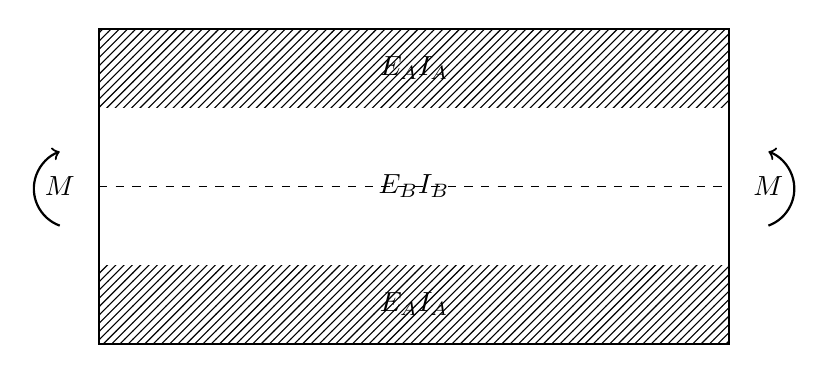
\begin{tikzpicture}

        % Draw the outer rectangle for the composite beam
        \draw[thick] (-4,-2) rectangle (4,2);

        % Draw the material A section (top and bottom) with shading
        \fill[pattern=north east lines] (-4,1) rectangle (4,2);
        \fill[pattern=north east lines] (-4,-2) rectangle (4,-1);

        % Label for E_A I_A at the top and bottom
        \node at (0,1.5) {$E_A I_A$};
        \node at (0,-1.5) {$E_A I_A$};

        % Label for E_B I_B in the middle
        \node at (0,0) {$E_B I_B$};

        % Draw the neutral axis (dashed line)
        \draw[dashed] (-4,0) -- (4,0);

        % Label for the bending moment M on both sides
        \node at (-4.5,0) {$M$};
        \node at (4.5,0) {$M$};

        % Draw the arrows indicating bending moment
        \draw[->,thick] (-4.5,-0.5) arc[start angle=250,end angle=110,radius=0.5];
        \draw[->,thick] (4.5,-0.5) arc[start angle=-70,end angle=70,radius=0.5];
    \end{tikzpicture}
    \caption{}
    \label{fig:9}
\end{figure}
\begin{multicols}{4}
    \begin{enumerate}
        \item $ \rho = \frac{E_A I_A + E_B I_B}{M} $
        \item $ \rho = \frac{E_B I_B + E_A I_A}{M} $
        \item $ \rho = \frac{M}{E_A I_A + E_B I_B} $
        \item $ \rho = \frac{(E_A + E_B)(I_A + I_B)}{M} $
    \end{enumerate}
\end{multicols}
\bigskip
\item Two pipes of constant sections but different diameters carry water at the same volume flow rate. The Reynolds number, based on the pipe diameter, is
\begin{multicols}{2}
    \begin{enumerate}
        \item $ \text{The same in both pipes} $
        \item $ \text{Larger in the narrower pipe} $
        \item $ \text{Smaller in the narrower pipe} $
        \item $ \text{Depends on the material of the pipes} $
    \end{enumerate}
\end{multicols}
\bigskip
\item Two airfoils of the same family are operating at the same angle of attack. The dimensions of one airfoil are twice as large as the other one. The ratio of the minimum pressure coefficient of the larger airfoil to the minimum pressure coefficient of the smaller airfoil is
\begin{multicols}{2}
    \begin{enumerate}
        \item $ 4.0 $
        \item $ 2.0 $
        \item $ 1.0 $
        \item $ 0.5 $
    \end{enumerate}
\end{multicols}
\bigskip
\item Wing $A$ has a constant chord $c$ and span $b$. Wing $B$ is identical but has a span $4b$. When both wings are operating at the same geometric angle of attack at subsonic speed, then:
    \begin{enumerate}
        \item $ \text{Wings A and B produce the same lift coefficient} $
        \item $ \text{Wing A produces a smaller lift coefficient than wing B} $
        \item $ \text{Wing A produces a greater lift coefficient than wing B} $
        \item $ \text{The freestream Mach number decides which wing produces the greater lift coefficient} $
    \end{enumerate}
\bigskip
\item A spring-mass-damper system is excited by a force $F_0 \sin \omega t$. The amplitude at resonance is measured to be $1$ cm. At half the resonant frequency, the amplitude is $0.5$ cm. The damping ratio of the system is
\begin{multicols}{2}
    \begin{enumerate}
        \item $ 0.1026 $
        \item $ 0.3242 $
        \item $ 0.7211 $
        \item $ 0.1936 $
    \end{enumerate}
\end{multicols}
\bigskip
\item The eigenvalues of the matrix\[A = \begin{bmatrix} 2 & 1 \\0 & 3\end{bmatrix}\]are
\begin{multicols}{4}
    \begin{enumerate}
        \item $ \text{1 and 2} $
        \item $ \text{1 and 3} $
        \item $ \text{2 and 3} $
        \item $ \text{2 and 4} $
    \end{enumerate}
\end{multicols}
\bigskip
\item The eigenvalues of the matrix $A^2$, where \[A = \begin{bmatrix} 2 & 1 \\0 & 3\end{bmatrix}\]
are
\begin{multicols}{2}
    \begin{enumerate}
        \item 1 and $\frac{1}{2}$
        \item 1 and $\frac{1}{3}$
        \item 2 and 3
        \item $\frac{1}{2}$ and $\frac{1}{3}$
    \end{enumerate}
\end{multicols}
\bigskip
\item The radius of the earth is $6.37 \times 10^6 \, \text{m}$ and the acceleration due to gravity at its surface is $9.81 \, \text{m/s}^2$. A satellite is in circular orbit at a height of $35.9 \times 10^6 \, \text{m}$ above the earth's surface. This orbit is inclined at $10.5^\circ$ degrees to the equator. The velocity change needed to make the orbit equatorial is:
    \begin{enumerate}
        \item $561 \, \text{m/s at } 84.75^\circ \text{ degrees to the initial direction}$
        \item $561 \, \text{m/s at } 95.25^\circ \text{ degrees to the initial direction}$
        \item $281 \, \text{m/s at } 84.75^\circ \text{ degrees to the initial direction}$
        \item $281 \, \text{m/s at } 95.25^\circ \text{ degrees to the initial direction}$
    \end{enumerate}
\bigskip
\item A piston-prop airplane having propeller efficiency, $\eta_p = 0.8$ and weighing $73108 \, \text{N}$ could achieve maximum climb rate of $15 \, \text{m/s}$ at flight speed of $50 \, \text{m/s}$. The excess Brake Power (BP) at the above flight condition will be:
\begin{multicols}{2}
    \begin{enumerate}
        \item $1700 \, \text{kW}$
        \item $2100 \, \text{kW}$
        \item $1371 \, \text{kW}$
        \item $6125 \, \text{kW}$
    \end{enumerate}
\end{multicols}
\bigskip
\item An airplane model with a symmetric airfoil was tested in a wind tunnel. $C_{m0}$ ($C_m$ at angle of attack, $\alpha = 0$) was estimated to be $0.08$ and $0$ respectively for elevator settings ($\delta_e$) of $5^\circ$ degrees up and $5^\circ$ degrees down. The estimated value of the elevator control power $\left(\frac{\partial C_m}{\partial \delta_e}\right)$ of the model will be:
\begin{multicols}{2}
    \begin{enumerate}
        \item $0.07 \, \text{per deg}$
        \item $-1.065 \, \text{per deg}$
        \item $-0.008 \, \text{per deg}$
        \item $-0.762 \, \text{per deg}$
    \end{enumerate}
\end{multicols}




